% Apertura del capítulo 9: paraboloide hiperbólico z = c·x·y con sus generatrices rectas.
% Compilar con: scripts/compilar_tikz.sh   (→ figures/svg/apertura-cap09-hypar.svg)
% Etiqueta: ilustrativa (malla de 20×20 celdas, proyección oblicua a mano; no es una figura de datos).
\def\pgfsysdriver{pgfsys-dvisvgm.def}
\documentclass[tikz,border=0pt]{standalone}
\usetikzlibrary{calc}
% PALETA-INICIO (generado por scripts/sincronizar_paleta.jl; no editar a mano)
\definecolor{azul}{HTML}{1B6CA8}
\definecolor{naranja}{HTML}{D95F02}
\definecolor{verde}{HTML}{2A9D8F}
\definecolor{gris}{HTML}{6B7280}
\definecolor{violeta}{HTML}{6F42C1}
\definecolor{ocre}{HTML}{8A5A00}
\definecolor{malla}{HTML}{CBD5E1}
% PALETA-FIN
\colorlet{lo}{verde}   % z mínimo
\colorlet{hi}{naranja}  % z máximo
\colorlet{fam1}{azul}  % generatrices θ¹ = cte
\colorlet{fam2}{violeta} % generatrices θ² = cte
\begin{document}
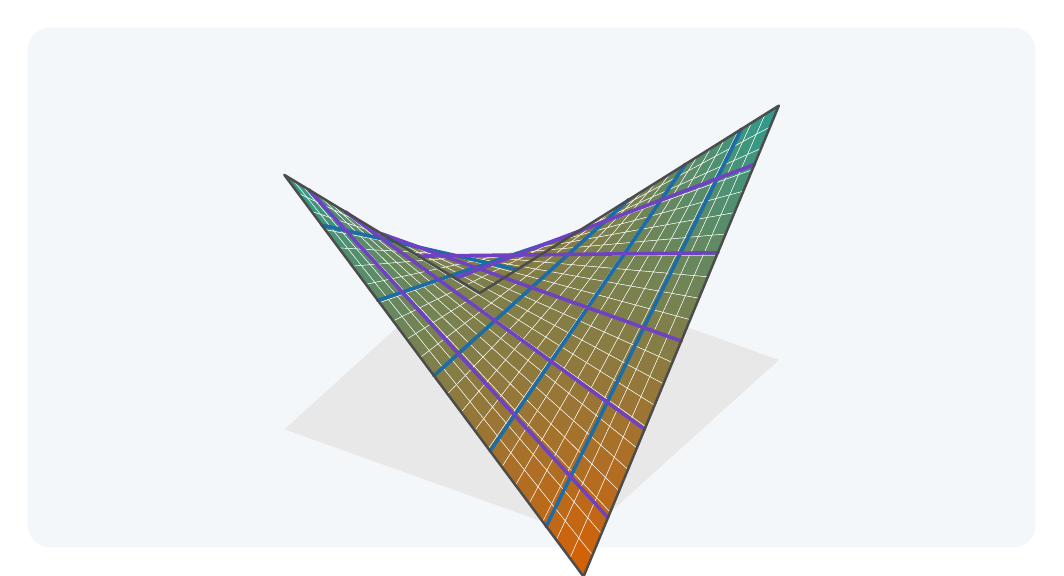
\begin{tikzpicture}[x={(0.95cm,-0.34cm)}, y={(0.62cm,0.56cm)}, z={(0cm,0.85cm)}, line join=round, line cap=round]
  \pgfmathsetmacro{\c}{0.55}   % z = c x y, x,y ∈ [-2,2]
  \pgfmathsetmacro{\L}{2.0}
  \pgfmathsetmacro{\N}{22}
  \pgfmathsetmacro{\h}{2*\L/\N}
  % Fondo tipo tarjeta (coordenadas de página)
  \useasboundingbox (canvas cs:x=-6.4cm,y=-3.3cm) rectangle (canvas cs:x=6.4cm,y=3.3cm);
  \fill[rounded corners=8pt, fill={rgb,255:red,244;green,247;blue,250}]
    (canvas cs:x=-6.4cm,y=-3.3cm) rectangle (canvas cs:x=6.4cm,y=3.3cm);
  % Sombra suave en el suelo (antes que la superficie)
  \fill[black!9] (-\L,-\L,-1.6) -- (\L,-\L,-1.6) -- (\L,\L,-1.6) -- (-\L,\L,-1.6) -- cycle;
  % Superficie: celdas de atrás hacia delante (y decreciente, x creciente)
  \foreach \j in {\numexpr\N-1\relax,...,0}{
    \foreach \i in {0,...,\numexpr\N-1\relax}{
      \pgfmathsetmacro{\xa}{-\L+\i*\h}
      \pgfmathsetmacro{\xb}{\xa+\h}
      \pgfmathsetmacro{\ya}{-\L+\j*\h}
      \pgfmathsetmacro{\yb}{\ya+\h}
      \pgfmathsetmacro{\zm}{\c*(\xa+\xb)*(\ya+\yb)/4}
      \pgfmathsetmacro{\t}{50+50*\zm/(\c*\L*\L)}
      \pgfmathsetmacro{\za}{\c*\xa*\ya}
      \pgfmathsetmacro{\zb}{\c*\xb*\ya}
      \pgfmathsetmacro{\zc}{\c*\xb*\yb}
      \pgfmathsetmacro{\zd}{\c*\xa*\yb}
      \fill[lo!\t!hi, draw=white, line width=0.15pt]
        (\xa,\ya,\za) -- (\xb,\ya,\zb) -- (\xb,\yb,\zc) -- (\xa,\yb,\zd) -- cycle;
    }
  }
  % Generatrices rectas: dos familias
  \foreach \u in {-1.5,-0.75,0,0.75,1.5}{
    \draw[fam1, line width=1.3pt] (\u,-\L,{\c*\u*(-\L)}) -- (\u,\L,{\c*\u*\L});
  }
  \foreach \v in {-1.5,-0.75,0,0.75,1.5}{
    \draw[fam2, line width=1.3pt] (-\L,\v,{\c*(-\L)*\v}) -- (\L,\v,{\c*\L*\v});
  }
  % Borde de la lámina
  \draw[black!70, line width=0.9pt] (-\L,-\L,{\c*\L*\L}) -- (\L,-\L,{-\c*\L*\L}) -- (\L,\L,{\c*\L*\L}) -- (-\L,\L,{-\c*\L*\L}) -- cycle;
\end{tikzpicture}
\end{document}
